\section{Implementation}

PQVRS is a big open source project (50K lines of code across C++, C\#, C for Graphic, Matlab, python, and some shell programing) and can be accessed at \cite{github}. Implementation of PQVRS is shown in Fig. \ref{implementation}. Compared with traditional video streaming system, several modules are newly added or modified, which are highlighted by pink color.

\begin{figure}
  \centering
  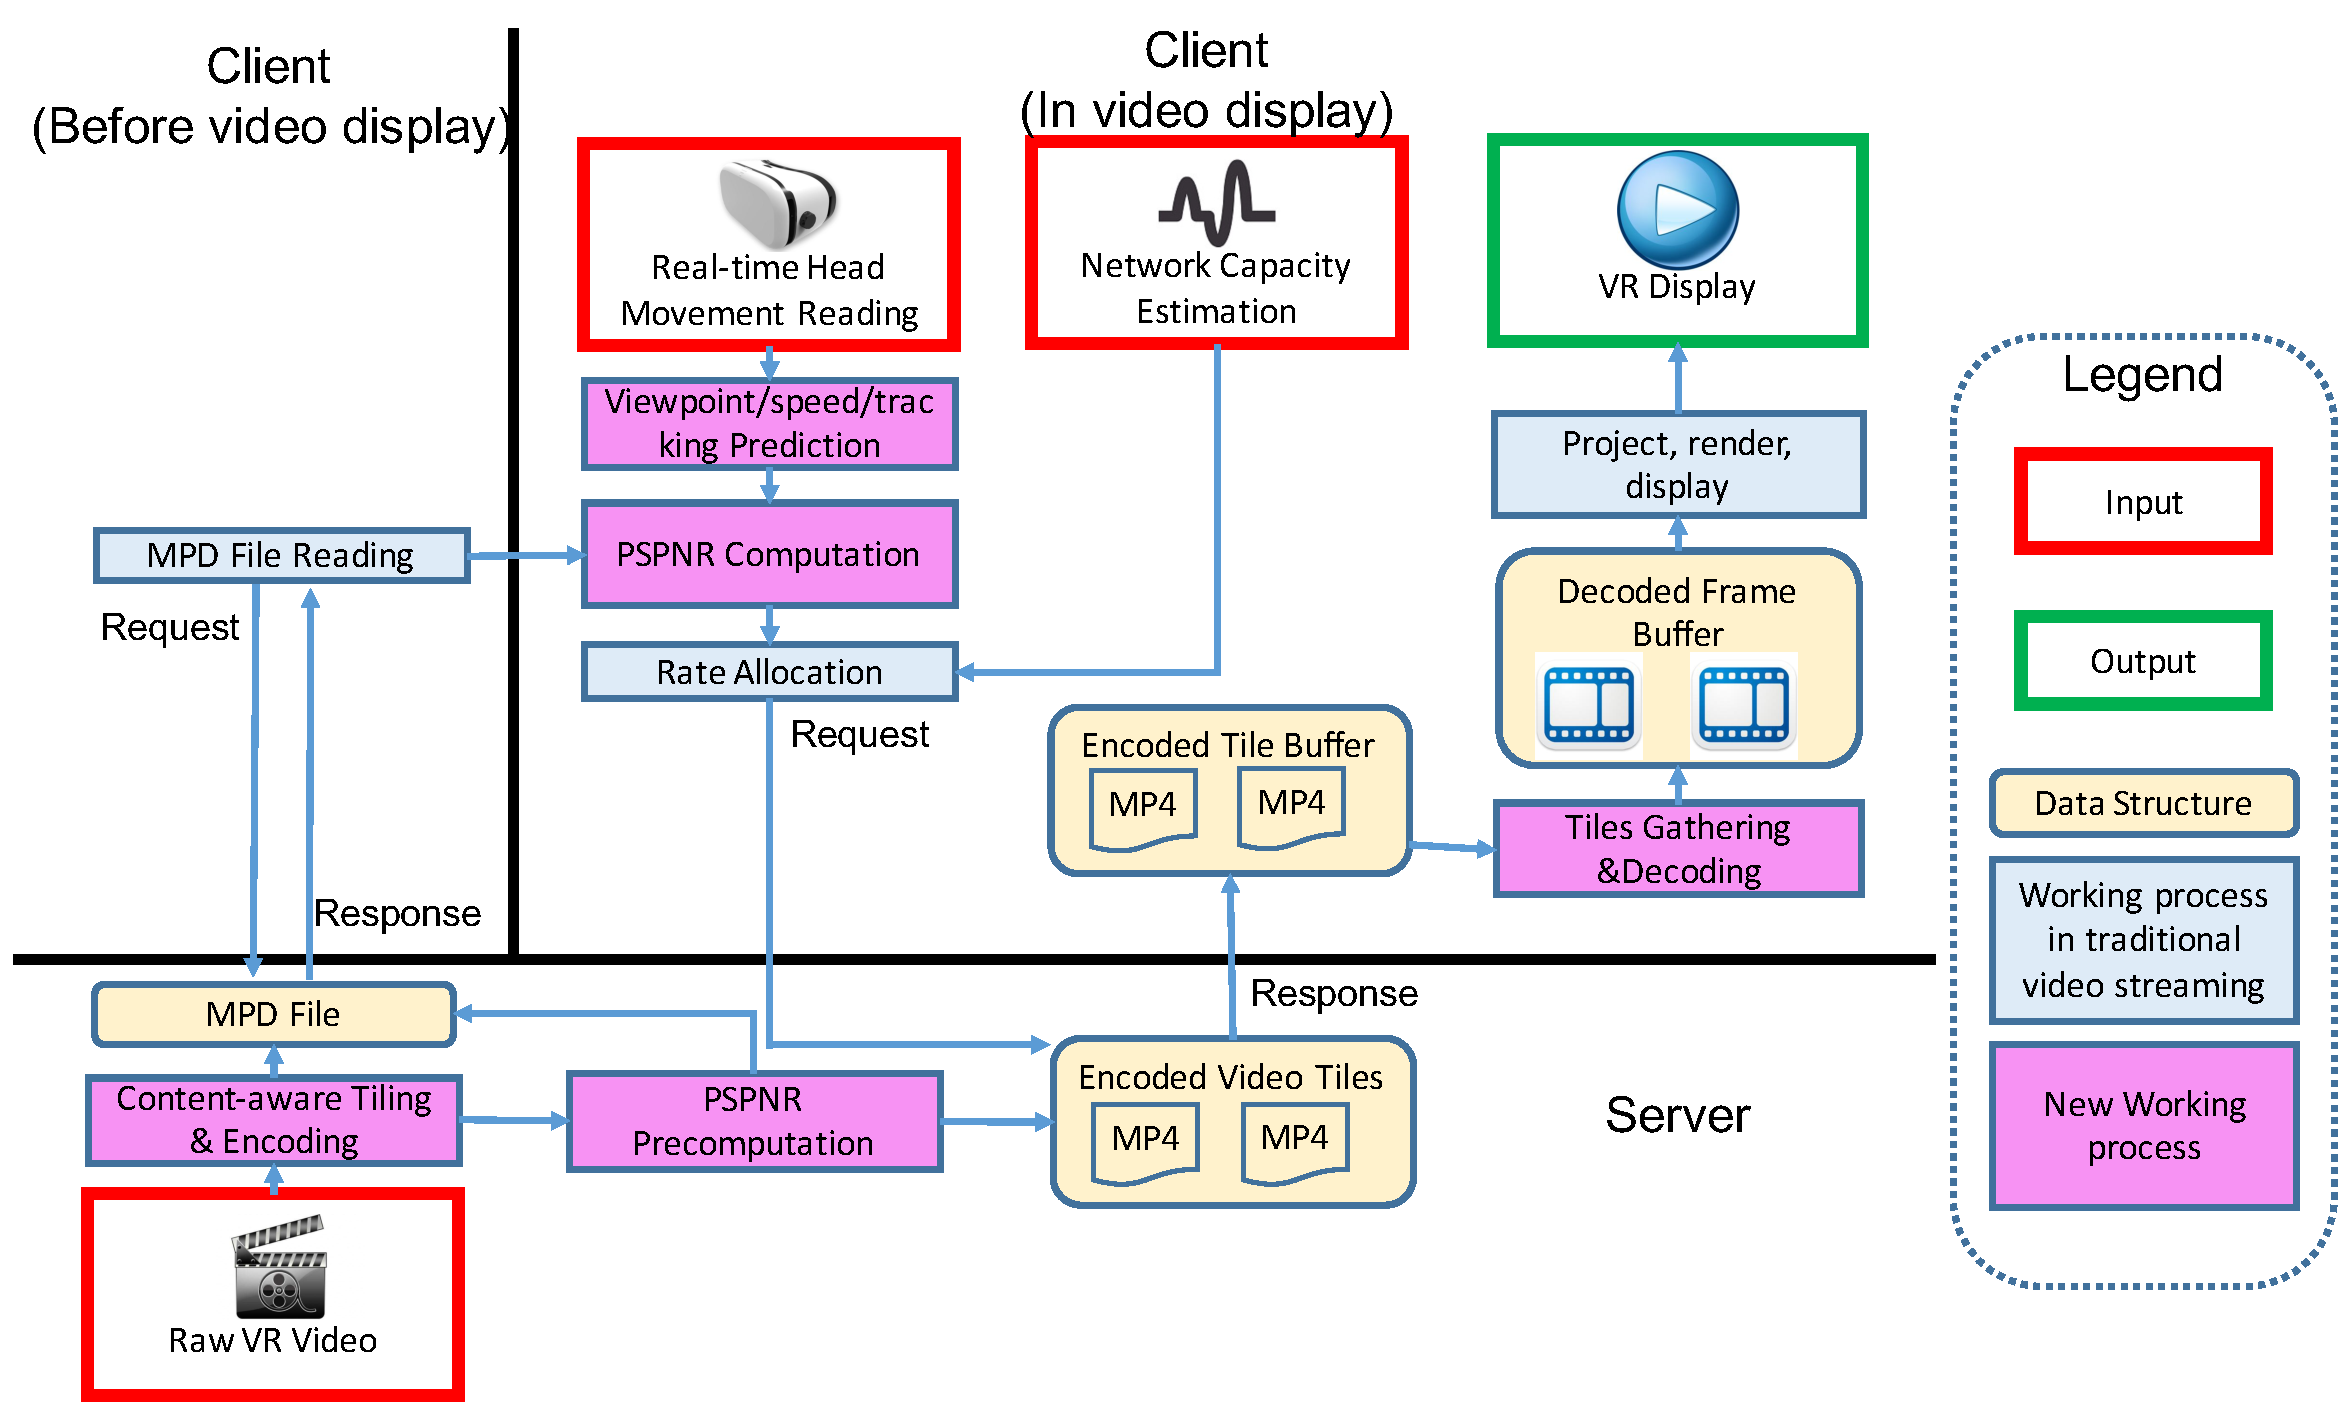
\includegraphics[width=3.5in]{images/implementation.pdf}
  \caption{Workflow of PQVRS.}
  \label{implementation}
  \end{figure}

\subsection{New component on Server-Side}

\textbf{Content-Aware Tiling / Encoding:} Based on our tiling algorithm described in Sec. 5, we cut each video segment into $N = 30$ rectangular tiles with different size. Each tile is encoded independently. The information of tiling result is packeted into MPD file so that client is aware of how each segment is cut. In addition, to prevent client-side stalling, we encode the lowest quality version of whole video without tiling, called "Base Layer".\cite{buffer} In real-time video streaming, client first request the Base Layer, then request the tiles with higher quality.

\textbf{PSPNR Precomputation:} Based on equation (\ref{f1}), (\ref{apprx_pmse}), server tries to compute PSPNR of each tile for 5 different BJNDs (1, 3, 5, 7, 9), then packet the result into MPD file. Compared with video content, size of this additional information is negligible.

\subsection{New component on Client-Side}

\textbf{Viewpoint / Speed / Tracking prediction:} In our system, viewpoint prediction is achieved by linear regression because of its efficiency and robustness. According to result of viewpoint prediction, we can estimate user's viewpoint moving speed by differentiating adjacent user viewpoints. Moreover, since we have analyzed object traces of video on server-side by YOLO \cite{yolo} and deliver the brief description to client-side, client-side can match the predictive viewpoint traces and object traces in order to predict if user is going to tracking an object.

\textbf{PSPNR Computation:} On client-side, based on our viewpoint / speed / tracking prediction, the value of BJND can be obtained by equation (\ref{BJND}). Then client read MPD file to get the PSPNR results with different BJNDs, and choose the one with the nearest BJND.

\textbf{Tiles Gathering \& Decoding:} For each video segment, client first decode the Base Layer. For tiles in user's viewport, we set up a multi-process decoder based on ffmpeg, and set up a buffer to cache the decoded frames of tiles to be played in the future. Specifically, the decoding scheduler dynamically selects a received tile and sends it to an idle decoder. The decoded frames are not necessarily consumed right away; instead they can be stored in the buffer residing in the video memory. When a cached frame is needed during the playback, its corresponding tiles are fed into GPU, then then mapping them from 2D to 3D for rendering on Head-Mounted Device.

\subsection{Other implementation details}
\textbf{MPD file: } In current Dynamic Adaptive Streaming over Http (DASH), MPD file includes many informations, such as resolution, frame rate, codecs, bandwidth. In Pano, we add 2 additional payload to MPD file: (1) tiling information and (2) PSPNR information. Tiling information includes each tile's width (8 bits integer), height (8 bits integer) and top left corner (8 bits integer for x axis and 8 bits integer for y axis), which measure data in the unit of 120 pixels. PSPNR information includes each tile's PSPNR value (16 bits float) in all 5 BJNDs and all 5 quality levels. The total size of our additional payload is only 1.5KB per second, which is negligible compared with actual streaming data size. (e.g. for a 5min VR video, the MPD size is only 450KB)

\textbf{Buffer: } We set up a double buffer system: a small-size Tile Buffer (5s, since we need to predict user's viewpoint / speed / tracking to determine quality of each tile, and prediction for >5s future is of poor accuracy) and a large-size Base Layer Buffer (30s, since requesting Base Layer does not need any prediction) \cite{buffer}. This double buffer system significantly reduces stalling, compared with only a 5s Tile Buffer \cite{Flare}.

\textbf{Project, render, display: }